\documentclass[a4paper, 10pt]{extarticle}

\usepackage[utf8]{inputenc}
\usepackage[russian]{babel}
\usepackage[
    paper=a4paper,
    left=15mm,
    right=15mm,
    top=0mm,
    bottom=10mm
]{geometry}
\usepackage{graphicx}
\usepackage{xcolor}
\usepackage{transparent}
\usepackage{changepage}
\usepackage{enumitem}
\usepackage{libertine}
\usepackage{fancyhdr}
\usepackage{paracol}
\usepackage{tcolorbox}
\usepackage{dashrule}
\usepackage{amssymb}
\usepackage[
    colorlinks=true,
    linkcolor=blue,
    citecolor=green,
    filecolor=magenta,
    urlcolor=blue
]{hyperref}

\newcommand{\Technologies}[1]{
    \begin{tcolorbox}[
        colback=blue!5,
        colframe=black,
        fonttitle=\bfseries,
        title=Технологии
    ]
    \texttt{\small{#1}}
    \end{tcolorbox}
}

\newcommand{\Scale}{1.25}
\tcbuselibrary{skins}

\linespread{1}
\setlength{\parindent}{1.25cm}
\setlength{\parskip}{1em}

\definecolor{blue}{HTML}{074799}
\definecolor{black}{HTML}{1A1A1D}

\pagestyle{empty}

\columnratio{0.35,0.65}
\setlength{\columnsep}{40pt}

\newcommand{\Sep}{
    \noindent\hdashrule[0.5ex]{\columnwidth}{1pt}{1mm 1pt}
}

\newcommand{\SubTitle}[2]{
    \parbox{1.75em}{
        \includegraphics[width=0.025\textwidth]{#1}
    }\textbf{\textit{\MakeUppercase{#2}}}
}

\newcommand{\ContactInfo}{
    \hspace{10.5em}\parbox{\columnwidth}{
        \begin{center}
            \SubTitle{img/human.png}{Контактная информация}
    
            \begin{tcolorbox}[
                enhanced,
                colframe=black,
                arc=5pt,
                left=1pt,
                right=1pt,
                top=2pt,
                bottom=2pt,
                halign=center,
                boxrule=0.5pt,
                hbox
            ]
                \begin{tabular}{ll}
                    \parbox{0.02\textwidth}{
                        
\includegraphics[width=0.02\textwidth]{img/phone.png}
                    } +7 (967) 281-53-04 &
                    \parbox{0.02\textwidth}{
                        
\includegraphics[width=0.02\textwidth]{img/mail.png}
                    } trud2004@yandex.ru \\
                    \parbox{0.02\textwidth}{
                        
\includegraphics[width=0.02\textwidth]{img/telegram.png}
                    } \href{https://t.me/Nep_pasha}{@Nep\_pasha} &
                    \parbox{0.02\textwidth}{
                        
\includegraphics[width=0.02\textwidth]{img/github.png}
                    } \href{https://github.com/nepavellab}{@nepavellab}
                \end{tabular}
            \end{tcolorbox}
        \end{center}
    }
}

\newcommand{\CVHat}{
\begin{adjustwidth}{-15mm}{-15mm}
    \colorbox{black}{
        \begin{minipage}[b][140pt][c]{\linewidth}
            \hspace{1.55cm}\parbox{0.1\textwidth}{
                \vspace{7em}
                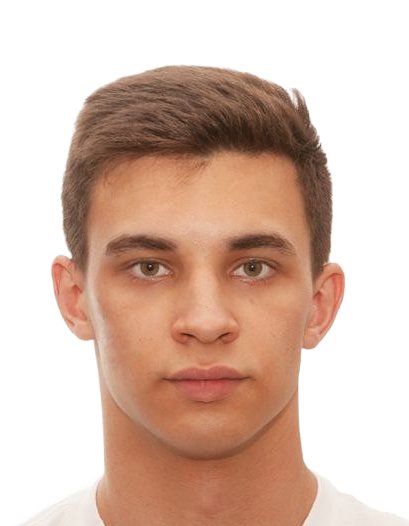
\includegraphics[width=0.24\columnwidth, height=0.3\textwidth]{img/profile.png}
            }
            \parbox{0.9\textwidth}{
                \begin{center}
                    \textcolor{white}{\huge{\transparent{0.7}{Программист}}}
                    \vspace{1em}

                    \textcolor{white}{\Huge{\textbf{НЕПОМНЯЩИХ \\ПАВЕЛ}}}
                \end{center}
            }
        \end{minipage}
    }
\end{adjustwidth}
\ContactInfo
}

\begin{document}
    \CVHat

    \begin{paracol}{2}
        \switchcolumn[0]
        \begin{leftcolumn}
            \Sep
            \begin{center}
                \SubTitle{img/skills.png}{Технические навыки}
            \end{center}
            \vspace{-1em}
            \begin{itemize}[
                label=\textcolor{black}{\scalebox{\Scale}{\textbullet}},
                topsep=0cm,
                leftmargin=0.275cm,
                itemsep=0.1cm
            ]
                \item Знание базовых алгоритмов \\и структур данных
                \item Опыт работы с параллельностью, \\многопоточностью и\\ асинхронностью
                \item Понимание архитектур\\ MVC, MVP и MVVM
                \item Опыт работы с базами данных\\ и сетевыми запросами
                \item Навыки с командной строкой\\ и системами контроля версий
            \end{itemize}
            
            \Sep
            \begin{center}
                \SubTitle{img/tech.png}{Стек технологий}
            \end{center}
            \vspace{-1em}
            \begin{itemize}[
                label=\textcolor{black}{\scalebox{\Scale}{\textbullet}}, 
                topsep=0cm,
                leftmargin=0.275cm,
                itemsep=0.1cm
            ]
                \item Основные языки: \\C/C++, Java, Kotlin
                \item SQLite, Firebase
                \item Android Framework
                \item Room
                \item Retrofit
                \item Dagger 2
                \item Jetpack Compose
            \end{itemize}

            \Sep
            \begin{center}
                \SubTitle{img/languages.png}{Языки}
            \end{center}
            \vspace{-1em}
            \begin{itemize}[
                label=\textcolor{black}{\scalebox{\Scale}{\textbullet}},
                topsep=0cm,
                leftmargin=0.275cm,
                itemsep=0.1cm
            ]
                \item Русский (носитель)
                \item Английский (B1)
            \end{itemize}
        \end{leftcolumn}

        \switchcolumn[1]
        \begin{rightcolumn}
            
            \Sep
            \begin{center}
                \SubTitle{img/education.png}{Образование}
            \end{center}
            \vspace{-1em}
            \noindent\parbox{0.1\columnwidth}{
                
\includegraphics[width=0.05\textwidth]{img/bmstu_logo.png}
            }
            \parbox{0.89\columnwidth}{
                \textbf{МГТУ им. Н.Э. Баумана}
                \hfill \textbf{Москва}
                \hrule
                \vspace{0.5em}

                Направление: \hfill \textit{2022 -- н.в.} 
                
                \textit{Математика и компьютерные науки}
            }

            \Sep
            \begin{center}
                \SubTitle{img/sec_edu.png}{Дополнительное образование}
            \end{center}
            \vspace{-1em}
            \noindent\parbox{0.09\columnwidth}{
                
\includegraphics[width=0.05\textwidth]{img/tbank_logo.png}
            }
            \parbox{0.9\columnwidth}{
                \textbf{НОЦ <<ДИЗРАПТ>> (Т-Банк \& МГТУ)}
                \hfill \textbf{Москва}
                \hrule
                \vspace{0.5em}

                Программа: \textit{Android разработчик}
                \hfill \textit{2024 -- 2024} 
            }
            \vspace{1em}

            \noindent\parbox{0.1\columnwidth}{
                
\includegraphics[width=0.05\textwidth]{img/vk_logo.png}
            }
            \parbox{0.89\columnwidth}{
                \textbf{ОЦ <<Технопарк>> (VK \& МГТУ)}
                \hfill \textbf{Москва}
                \hrule
                \vspace{0.5em}

                Программа: \textit{Android разработчик}
                \hfill \textit{2024 -- н.в.} 
            }

            \Sep
            \begin{center}
                \SubTitle{img/project.png}{Проектная деятельность}
            \end{center}
            \vspace{-1em}
            \textcolor{blue}{$\blacktriangleright$}
            \textbf{\underline{Приложение для организации мероприятий}}
            
            \Technologies{Java, ZXing, Firebase, Android Framework}
            
            \noindent Разработал мобильное приложения для создания мероприятий.
            Создал авторизацию через сторонние сервисы, функцию восстановление пароля через почту,
            реализовал работу с QR через камеру, добавление и считывание данных из базы по сети.
            
            \noindent\textcolor{blue}{$\blacktriangleright$} 
            \textbf{\underline{Веб-сервис <<вопрос-ответ>> (в рамках курса ОЦ <<Технопарк>>)}}
        
            \Technologies{JavaScript, Python, Django, HTML \& CSS, Bootstrap, PostgreSQL}
            
            \noindent Разработал веб-сайт (аналог <<Stack Overflow>>) для обсуждения проблем различной тематики.

            \noindent\textcolor{blue}{$\blacktriangleright$}
            \noindent\textbf{\underline{Инструменты в проектах в ходе учебной деятельности}}
            
            \Technologies{OpenMP, Qt/PyQt, numpy, Three.js, LaTeX, bash}

        \end{rightcolumn}
    \end{paracol}
    \vspace{1em}

    \noindent\rule{\textwidth}{1.25pt}
\end{document}